\section{Đề số 36}

\begin{bt} 
	\hfill
	\begin{enumerate}[a.]
		\item Cho a, b, c là ba số thực dương thỏa mãn điều kiện: $\frac{a+b-c}{c}=\frac{b+c-a}{a}=\frac{c+a-b}{b}$. \\[5px]Hãy tính giá trị của biểu thức: $B=\left(1+\frac{b}{a}\right)\left(1+\frac{a}{c}\right)\left(1+\frac{c}{b}\right)$.
		\item Cho tỉ lệ thức $\frac{a}{b}=\frac{c}{d}$ với $a \neq 0, b \neq 0, c \neq 0, d \neq 0, a \neq \pm b, c \neq \pm d$.
		\\[5px]Chứng minh: $\left(\frac{a-b}{c-d}\right)^{2013}=\frac{a^{2013}+b^{2013}}{c^{2013}+d^{2013}}$
	\end{enumerate}
	
	\loigiai{
		\begin{enumerate}
			\item Cho a, b, c là ba số thực dương thỏa mãn điều kiện:\\[5px]
			$\frac{a+b-c}{c}=\frac{b+c-a}{a}=\frac{c+a-b}{b}$\\[5px]
			Hãy tính giá trị của biểu thức: $B=\left(1+\frac{b}{a}\right)\left(1+\frac{a}{c}\right)\left(1+\frac{c}{b}\right)$\\[5px]
			Vì $\mathrm{a}, \mathrm{b}, \mathrm{c}$ là các số dương nên $a+b+c \neq 0$\\[5px]
			Theo tính chất dãy tỉ số bằng nhau ta có:\\[5px]
			$\frac{a+b-c}{c}=\frac{b+c-a}{a}=\frac{c+a-b}{b}=\frac{a+b-c+b+c-a+c+a-b}{a+b+c}=1 \\[5px]
			\text { Nên: } \frac{a+b-c}{c}+1=\frac{b+c-a}{a}+1=\frac{c+a-b}{b}+1=2 \\[5px]
			\Rightarrow \frac{a+b}{c}=\frac{b+c}{a}=\frac{c+a}{b}=2$\\[5px] 
			Mà $B=\left(1+\frac{b}{a}\right)\left(1+\frac{a}{c}\right)\left(1+\frac{c}{b}\right) \\[5px]
			\Rightarrow B=\left(\frac{a+b}{a}\right)\left(\frac{c+a}{c}\right)\left(\frac{b+c}{b}\right)=8$\\[5px]
			Vậy: $B=8$
			\item Cho tỉ lệ thức $\frac{a}{b}=\frac{c}{d}$ với $a \neq 0, b \neq 0, c \neq 0, d \neq 0, a \neq \pm b, c \neq \pm d$.\\[5px]
			Chứng minh: $\left(\frac{a-b}{c-d}\right)^{2013}=\frac{a^{2013}+b^{2013}}{c^{2013}+d^{2013}}$\\[5px]
			Ta có: $\frac{a}{b}=\frac{c}{d}=\frac{a-c}{b-d} \Rightarrow\left(\frac{a}{b}\right)^{2013}=\left(\frac{c}{d}\right)^{2013}=\left(\frac{a-c}{b-d}\right)^{2013}$\\[5px]
			Mà: $\left(\frac{a}{b}\right)^{2013}=\left(\frac{c}{d}\right)^{2013}=\frac{a^{2013}}{b^{2013}}=\frac{c^{2013}}{d^{2013}}=\frac{a^{2013}+c^{2013}}{b^{2013}+d^{2013}}$\\[5px]
			Từ (1) và $(2) \Rightarrow\left(\frac{a-b}{c-d}\right)^{2013}=\frac{a^{2013}+b^{2013}}{c^{2013}+d^{2013}} \quad$ (đpcm)
		\end{enumerate}
	} 
\end{bt}

\begin{bt}
	\hfill
	\begin{enumerate}[a.]
		\item Cho $\frac{x}{y+z+t}=\frac{y}{z+t+x}=\frac{z}{t+x+y}=\frac{t}{x+y+z}$
		\\[5px]Chứng minh rằng: Biểu thức sau có giá trị nguyên
		$$
		A=\frac{x+y}{z+t}+\frac{y+z}{t+x}+\frac{z+t}{x+y}+\frac{t+x}{y+z}
		$$
		\item Tìm $x$ biết: $x^2-5 x+6=0$
		\item Số $\mathrm{A}$ được chia thành ba phần số tỉ lệ theo $\frac{2}{5}: \frac{3}{4}: \frac{1}{6}$. Biết rằng tổng các bình phương của ba số đó bằng 24309 . Tìm số $\mathrm{A}$.
	\end{enumerate}
	\loigiai{
		\begin{enumerate}
			\item Cho $\frac{x}{y+z+t}=\frac{y}{z+t+x}=\frac{z}{t+x+y}=\frac{t}{x+y+z}$\\[5px]
			Chứng minh rằng: Biểu thức sau có giá trị nguyên\\[5px]
			$$
			A=\frac{x+y}{z+t}+\frac{y+z}{t+x}+\frac{z+t}{x+y}+\frac{t+x}{y+z}
			$$
			Ta có: $\frac{x}{y+z+t}=\frac{y}{z+t+x}=\frac{z}{t+x+y}=\frac{t}{x+y+z}=\frac{x+y+z+t}{3(x+y+z+t)}=\frac{1}{3}$\\[5px]
			$\Rightarrow 3 x=y+z+t ; 3 y=z+t+x ; 3 z=t+x+y ; 3 t=x+y+z \\[5px]
			\Rightarrow x+y=z+t ; y+z=t+x ; z+t=x+y ; t+x=y+z \\[5px]
			\Rightarrow A=\frac{x+y}{z+t}+\frac{y+z}{t+x}+\frac{z+t}{x+y}+\frac{t+x}{y+z}=1+1+1+1=4 \in Z$\\[5px]
			Vậy biểu thức A có giá trị nguyên. (đpcm)
			\item Tìm $x$ biết: $x^2-5 x+6=0$\\[5px]
			Ta có: $x^2-3 x-2 x+6=0$\\[5px]
			$\Leftrightarrow\left(x^2-3 x\right)-(2 x-6)=0 \\[5px]
			\Leftrightarrow x(x-3)-2(x-3)=0 \\[5px]
			\Leftrightarrow(x-3)(x-2)=0 \\[5px]
			\Leftrightarrow\left[\begin{array} { l } 
			{ x - 3 = 0 } \\[5px]
			{ x - 2 = 0 }
			\end{array} \Leftrightarrow \left[\begin{array}{l}
			x=3 \\[5px]
			x=2
			\end{array}\right.\right.$\\[5px]
			Vậy: $x=2$ hoặc $x=3$
			\item Số $\mathrm{A}$ được chia thành ba phần số tỉ lệ theo $\frac{2}{5}: \frac{3}{4}: \frac{1}{6}$.\\[5px] Biết rằng tổng các bình phương của ba số đó bằng 24309 . Tìm số $\mathrm{A}$.\\[5px]
			Gọi ba phân được chia lần lượt là: $a, b, c$\\[5px]
			Theo bài ra ta có: $a: b: c=\frac{2}{5}: \frac{3}{4}: \frac{1}{6}$ và $a^2+b^2+c^2=24309$\\[5px]
			Ta có: $a: b: c=\frac{2}{5}: \frac{3}{4}: \frac{1}{6}=24: 45+10 \Rightarrow \frac{a}{24}=\frac{b}{45}=\frac{c}{10}$\\[5px]
			Áp dụng tính chất dãy tỉ số bằng nhau ta có:\\[5px]
			$\frac{a}{24}=\frac{b}{45}=\frac{c}{10} \Rightarrow \frac{a^2}{576}=\frac{b^2}{2025}=\frac{c^2}{100}=\frac{a^2+b^2+c^2}{576+2025+100}=\frac{24309}{2701}=9 \\[5px]
			\Rightarrow a^2=576.9=5184 \Rightarrow a= \pm 72 \\[5px]
			b^2=2025.9=18225 \Rightarrow b= \pm 135 \\[5px]
			c^2=100.9=900 \Rightarrow c=30 \\[5px]
			\text {Vì: } \frac{a}{24}=\frac{b}{45}=\frac{c}{10} \Rightarrow \mathrm{a}, \mathrm{b}, \mathrm{c} \text { cùng dấu. } \\[5px]
			\Rightarrow A=-72+(-135)+(-30)=-237 \\[5px]
			A=72+135+30=235$\\[5px]
			Vậy: $A=-135$ hoặc $A=135$
		\end{enumerate}
	} 
\end{bt}

\begin{bt}
	Tìm giá trị nhỏ nhất của biểu thức: $A=|x-2013|+|x-3014|+|x-2015|$
	\loigiai{
		Tìm giá trị nhỏ nhất của biểu thức:\\[5px]
		$A= |x-2013|+|x-3014|+|x-2015| \\[5px]
		\text {Ta có: }|x-2015|=|2015-x| \\[5px]
		\Rightarrow A=(|x-2013|+|2015-x|)+|x-3014| \\[5px]
		\Rightarrow A \geq|x-2013+2015-x|+|x-2014| \\[5px]
		\Rightarrow A \geq 2+|x-2014| \\[5px]
		\text {Mà: }|x-3014| \geq 0 \\[5px]
		\Rightarrow A \geq 0 \\[5px]
		\text {Dấu bằng xảy ra } \Leftrightarrow\left\{\begin{array} { l } 
		{ ( x - 2 0 1 3 ) ( 2 0 1 5 - x ) } \\[5px]
		{ x = 2 0 1 4 }
		\end{array} \Leftrightarrow \left\{\begin{array}{l}
		2013 \leq x \leq 2014 \\[5px]
		x=2014
		\end{array}\right.\right. \\[5px]
		\Leftrightarrow x=2014$
		Vậy GTNN của A là 2 khi $x=2014$
	} 
\end{bt}

\begin{bt}
	Tìm hai số dương biết tổng, hiệu, tích của chúng tỉ lệ nghịch với ba số 20;120;16.
	\loigiai{
		Tìm hai số dương biết tổng hiệu tích của chúng tỉ lệ nghịch với ba số 30; 120; 16.\\[5px] 
		Gọi hai số dương cần tìm là $x, y$\\[5px] 
		Theo bài ra ta có: $30(x+y)=120(x-y)=16 x y$\\[5px]
		$\Rightarrow \frac{x+y}{8}=\frac{x-y}{2}=\frac{x y}{15}=k \\[5px]
		\Rightarrow x+y=8 k ; x-y=2 k ; x y=15 k \\[5px]
		\Rightarrow x=5 k ; y=3 k \Rightarrow x y=5 k \cdot 3 k=15 k \\[5px]
		15 k^2=15 k \Rightarrow k=1 \\[5px]
		\Rightarrow x+y=8 ; x-y=2 \Rightarrow x=5 ; y=3$\\[5px]
		Vậy hai số dương cần tìm là 5 và 3 .
	}
\end{bt}

\begin{bt}
	Cho tam giác $\mathrm{ABC}$ vuông ở $\mathrm{A}$, có góc $C=30^{\circ}$, đường cao $\mathrm{AH}$. Trên đoạn $\mathrm{HC}$ lấy điểm $\mathrm{D}$ sao cho $H D=H B$. Từ $\mathrm{C}$ kẻ $\mathrm{CE}$ vuông góc với $\mathrm{AD}$. Chứng minh:
	\begin{enumerate}[a.]
		\item Tam giác $\mathrm{ABD}$ là tam giác đều.
		\item $A H=C E$.
		\item HE song song với $A C$.
	\end{enumerate}
	\loigiai{
		$$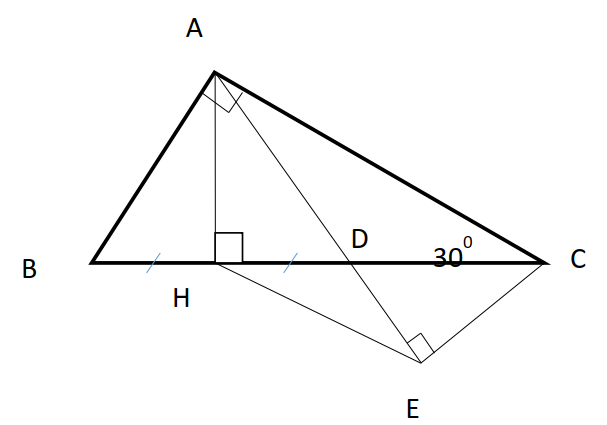
\includegraphics[width=0.5\textwidth]{36-5-lg.png}$$
		\begin{enumerate}
			\item $\triangle A B D$ có $\mathrm{AH}$ vừa là đường cao vừa là đường trung tuyến nên $\triangle A B D$ cân tại $\mathrm{A}$.\\[5px]
			Ta có: $B+C=90^{\circ}$ (Hai góc nhọn của một tam giác vuông)\\[5px]
			$\Rightarrow B=90^{\circ}-30^{\circ}=60^{\circ}$\\[5px]
			Nên $\triangle A B D$ là tam giác đều. (đpcm)
			\item Ta có: $E A C=B A C-A B D=90^{\circ}-60^{\circ}=30^{\circ}$\\[5px]
			$\Rightarrow \triangle A H C=\triangle C E A$ (cạnh huyền -góc nhọn)\\[5px]
			Do đó $\mathrm{AH}=\mathrm{CE}$ (đpcm)
			\item$\triangle A H C=\triangle C E A(\mathrm{cmt})$ nên $\mathrm{HC}=\mathrm{EA}(1)$\\[5px]
			$\triangle A D C$ cân ở $\mathrm{D}$ vì có $A D C=D C A=30^{\circ} \Rightarrow \triangle D A C$ cân ở $\mathrm{D}$.\\[5px]
			Suy ra $: \mathrm{DA}=$ DC. (2)\\[5px]
			Từ (1) và (2) $\Rightarrow D H=D E \Rightarrow \triangle D H E$ cân tại $\mathrm{D}$\\[5px]
			Hai tam giác cân ADC và $\mathrm{DEH}$ có:\\[5px] 
			Hai tam giác cân: $\triangle A C D$ cân tại $\mathrm{D}$ và $\triangle D H E$ cân tại $\mathrm{D}$ có:\\[5px] 
			$A D C=H D E(\text{đđ}) \Rightarrow D H E=A D C$ ở vị trí so le trong\\[5px] 
			$\Rightarrow E H / / A C$ (đpcm)
		\end{enumerate}
	}
\end{bt}


